\section{Technical Details}

\frame{\tableofcontents[currentsection]}

\begin{frame}
  \frametitle{Implementation Goals}
  \begin{itemize}
    \item Our implementation will not focus on speed
    \item We prioritise ease of implementation
    \item Step by step approach
  \end{itemize}
\end{frame}

\begin{frame}
  \frametitle{Overview}
  \begin{center}
    \begin{tikzpicture}[milestone/.style={drop shadow,draw,fill=red!50,minimum height=7.5mm,minimum width=1cm,font=\tiny\scshape},
                        link/.style={-latex,thick},
                        arrow/.style={blue,ultra thick,-{Stealth[]}},
                        scale=.8,transform shape]
      \node[milestone] (uint8) at (0,0) {\texttt{Stream<uint8>}};
      \node[milestone] (wave) at ($ (uint8) + (3,0) $) {\texttt{Wave}};

      \foreach[count=\y from 1] \x in {0xA1,0x14,0x73,0x9C} {
        \node[minimum width=8mm,minimum height=5mm,font=\tiny\scshape,draw,anchor=south] at ($ (uint8.north) + (0,\y*0.5) $) {\x};
      }

      \begin{scope}[xshift=2cm,yshift=1.875cm]
        \draw (0,-1) rectangle (2,1);
        \draw[thin] plot[domain=0:360,x=0.00555cm,y=5mm,samples=100,smooth] (\x,{sin(\x)+0.2*sin(4*\x)});
      \end{scope}

      \draw[link] (uint8) -- (wave);

      \visible<1>{
        \draw[arrow] ($ (uint8) - (0,1.5) $) -- (uint8);
      }
      \visible<2>{
        \draw[arrow] ($ (wave) - (0,1.5) $) -- (wave);
      }
    \end{tikzpicture}
  \end{center}
  \begin{overprint}
    \onslide<1>
    \begin{itemize}
      \item The WAV file contains raw bytes (\texttt{uint8\_t})
      \item This is what we start with
      \item A \texttt{Stream} is basically just a list
            \begin{itemize}
              \item \texttt{stream[i]} gives \texttt{i}-th byte
            \end{itemize}
      \item This raw format is not easy to work with
    \end{itemize}
    \onslide<2>
    \begin{itemize}
      \item We want to construct with a \texttt{Wave}
      \item I.e.~a \texttt{double function(double)}
      \item Much easier to work with
      \item Multiple steps necessary to get there
    \end{itemize}
  \end{overprint}
\end{frame}

\subsection{Samples}

\frame{\tableofcontents[currentsubsection]}

\begin{frame}
  \frametitle{WAV Files}
  \begin{itemize}
    \item In essence, a WAV file is a series of values which represent the amplitudes of a wave
  \end{itemize}
  \begin{center}
    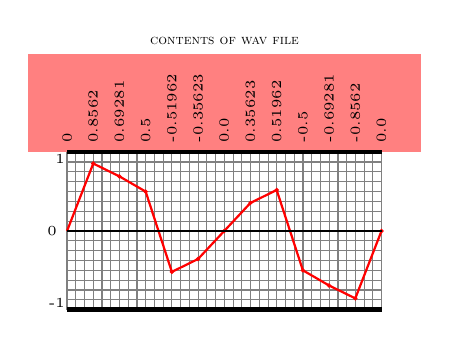
\begin{tikzpicture}
      \path[fill=red!50] (-0.5,1) rectangle (4.5,2.25);
      \node[anchor=south,font=\scshape\tiny] at (2,2.25) {contents of wav file};

      \draw[thin,gray] (0,-1) grid[xstep=0.111cm,ystep=0.125cm] (4,1);

      \foreach[evaluate={0.7*sin(2*\x)+0.2*sin(5*\x)+0.3*sin(13*\x)} as \y,
               remember=\y as \lasty (initially 0),
               remember=\x as \lastx (initially 0)] \x in {30,60,...,360} {
        \draw[fill,red] (\x*0.0111,\y) circle [radius=0.02cm];
        \node[right,font=\tiny,rotate=90] at (\x*0.0111,1) {\y};
        \draw[thick,red] (\lastx*0.0111,\lasty) -- (\x*0.0111,\y);
      }

      \node[right,font=\tiny,rotate=90] at (0,1) {0};

      \draw[ultra thick] (0,1) -- (4,1) node[at start,anchor=north east,inner sep=0pt,font=\tiny] {1};
      \draw[thick] (0,0) -- (4,0) node[at start,anchor=east,font=\tiny] {0};
      \draw[ultra thick] (0,-1) -- (4,-1) node[at start,anchor=south east,inner sep=0pt,font=\tiny] {-1};
    \end{tikzpicture}
  \end{center}
\end{frame}

\begin{frame}
  \frametitle{WAV Files}
  \begin{itemize}
  \item However, WAV files do not use floating points numbers
    \item WAV files use integers
    \item They range from 0 to 255 for 8 bit WAVs
    \item Or \num{-32768} to \num{+32768} for 16 bit WAVs
  \end{itemize}
  \begin{overprint}
    \onslide<1>
    \begin{center}
      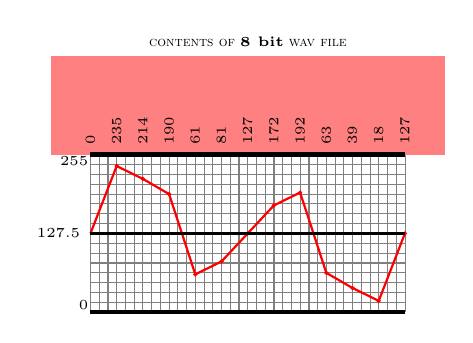
\begin{tikzpicture}
        \path[fill=red!50] (-0.5,1) rectangle (4.5,2.25);
        \node[anchor=south,font=\scshape\tiny] at (2,2.25) {contents of \textbf{8 bit} wav file};

        \draw[thin,gray] (0,-1) grid[xstep=0.111cm,ystep=0.125cm] (4,1);

        \foreach[evaluate={0.7*sin(2*\x)+0.2*sin(5*\x)+0.3*sin(13*\x)} as \y,
                 remember=\y as \lasty (initially 0),
                 remember=\x as \lastx (initially 0),
                 evaluate={int(\y*127+127)} as \v] \x in {30,60,...,360} {
          \draw[fill,red] (\x*0.0111,\y) circle [radius=0.02cm];
          \node[right,font=\tiny,rotate=90] at (\x*0.0111,1) {\v};
          \draw[thick,red] (\lastx*0.0111,\lasty) -- (\x*0.0111,\y);
        }

        \node[right,font=\tiny,rotate=90] at (0,1) {0};

        \draw[ultra thick] (0,1) -- (4,1) node[at start,anchor=north east,inner sep=0pt,font=\tiny] {255};
        \draw[thick] (0,0) -- (4,0) node[at start,anchor=east,font=\tiny] {127.5};
        \draw[ultra thick] (0,-1) -- (4,-1) node[at start,anchor=south east,inner sep=0pt,font=\tiny] {0};
      \end{tikzpicture}
    \end{center}
    \onslide<2>
    \begin{center}
      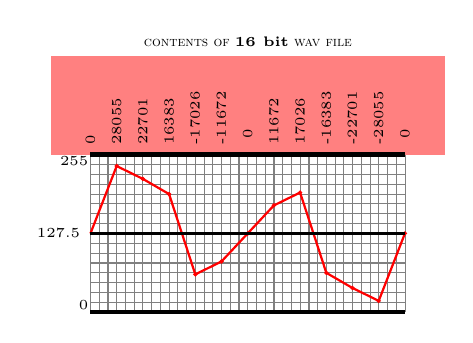
\begin{tikzpicture}
        \path[fill=red!50] (-0.5,1) rectangle (4.5,2.25);
        \node[anchor=south,font=\scshape\tiny] at (2,2.25) {contents of \textbf{16 bit} wav file};

        \draw[thin,gray] (0,-1) grid[xstep=0.111cm,ystep=0.125cm] (4,1);

        \foreach[evaluate={0.7*sin(2*\x)+0.2*sin(5*\x)+0.3*sin(13*\x)} as \y,
                 remember=\y as \lasty (initially 0),
                 remember=\x as \lastx (initially 0),
                 evaluate={\y*32.767} as \v,
                 evaluate={int(\v)} as \thousands,
                 evaluate={int(abs(\v-\thousands)*1000)} as \rest] \x in {30,60,...,360} {
          \draw[fill,red] (\x*0.0111,\y) circle [radius=0.02cm];
          \node[right,font=\tiny,rotate=90] at (\x*0.0111,1) {\ifnum\thousands=0
                                                                {}
                                                              \else\thousands\fi
                                                              \ifnum\rest=0
                                                                0
                                                              \else
                                                              \ifnum\rest<10 00\rest
                                                              \else\ifnum\rest<100 0\rest
                                                                         \else\rest\fi\fi\fi};
          \draw[thick,red] (\lastx*0.0111,\lasty) -- (\x*0.0111,\y);
        }

        \node[right,font=\tiny,rotate=90] at (0,1) {0};

        \draw[ultra thick] (0,1) -- (4,1) node[at start,anchor=north east,inner sep=0pt,font=\tiny] {255};
        \draw[thick] (0,0) -- (4,0) node[at start,anchor=east,font=\tiny] {127.5};
        \draw[ultra thick] (0,-1) -- (4,-1) node[at start,anchor=south east,inner sep=0pt,font=\tiny] {0};
      \end{tikzpicture}
    \end{center}
  \end{overprint}
\end{frame}

\begin{frame}
  \frametitle{Overview Update}
  \begin{center}
    \begin{tikzpicture}[milestone/.style={drop shadow,draw,fill=red!50,minimum height=7.5mm,minimum width=1cm,font=\tiny\scshape},
                        link/.style={-latex,thick},
                        arrow/.style={blue,ultra thick,-{Stealth[]}},
                        scale=.8,transform shape]
      \node[milestone] (uint8) at (0,0) {\texttt{Stream<uint8>}};
      \node[milestone] (int16) at ($ (uint8) + (2,1) $) {\texttt{Stream<int16>}};
      \node[milestone] (double) at ($ (uint8) + (4,0) $) {\texttt{Stream<double>}};
      \node[milestone] (wave) at ($ (double) + (3,0) $) {\texttt{Wave}};

      \draw[link] (uint8) |- (int16);
      \draw[link] (int16) -| (double);
      \draw[link] (uint8) -- (double);
      \draw[link] (double) -- (wave);

      \visible<1>{
        \coordinate (link middle) at ($ (uint8.east) ! 0.5 ! (double.west) $);
        \draw[arrow] ($ (link middle) - (0,1.5) $) -- (link middle);
      }
      \visible<2>{
        \draw[arrow] ($ (int16) + (0,1.5) $) -- (int16);
      }
    \end{tikzpicture}
  \end{center}
  \begin{overprint}
    \onslide<1>
    \begin{itemize}
      \item If the WAV file contains 8 bit samples, we can directly convert them to \texttt{double}s
      \item Convert $[0,255]$ to $[-1,1]$
            \begin{center}
              \texttt{byte / 127.5 - 1}
            \end{center}
    \end{itemize}

    \onslide<2>
    \begin{itemize}
      \item If the WAV file contains 16 bit samples, however, we must first group pairs of bytes together to
            form the 16 bit values
            \begin{center} \ttfamily
              sample = byte1 | (byte2 << 8) 
            \end{center}
      \item Convert $[0,255]$ to $[-1,1]$
            \begin{center} \ttfamily
              sample / 32768.0
            \end{center}
    \end{itemize}
  \end{overprint}
\end{frame}



%%% Local Variables:
%%% mode: latex
%%% TeX-master: "sound"
%%% End:

\subsection{Interpolation}

\frame{\tableofcontents[currentsubsection]}

\begin{frame}
  \frametitle{Interpolation}
  \begin{center}
    \begin{tikzpicture}[milestone/.style={drop shadow,draw,fill=red!50,minimum height=7.5mm,minimum width=1cm,font=\tiny\scshape},
                        link/.style={-latex,thick},
                        arrow/.style={blue,ultra thick,-{Stealth[]}},
                        scale=.8,transform shape]
      \node[milestone] (uint8) at (0,0) {\texttt{Stream<uint8>}};
      \node[milestone] (int16) at ($ (uint8) + (2,1) $) {\texttt{Stream<int16>}};
      \node[milestone] (double) at ($ (uint8) + (4,0) $) {\texttt{Stream<double>}};
      \node[milestone] (wave) at ($ (double) + (3,0) $) {\texttt{Wave}};

      \draw[link] (uint8) |- (int16);
      \draw[link] (int16) -| (double);
      \draw[link] (uint8) -- (double);
      \draw[link] (double) -- (wave);

      
      \coordinate (link middle) at ($ (double.east) ! 0.5 ! (wave.west) $);
      \draw[arrow] ($ (link middle) - (0,1.5) $) -- (link middle);
    \end{tikzpicture}
  \end{center}
  \begin{itemize}
    \item \texttt{Stream<double>} is a sequence of discrete values (red)
    \item We want to construct a continuous curve (blue)
  \end{itemize}
  \begin{center}
    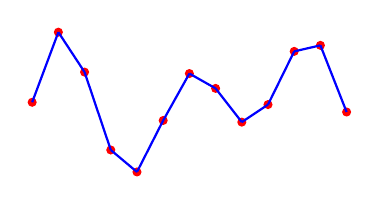
\begin{tikzpicture}
      \draw[fill,red] (0,0) circle [radius=0.05cm];
      \foreach[count=\i,
               evaluate={sin(2.5*\x) * 0.6 + cos(1.3*\x) * 0.4} as \y,
               remember=\y as \lasty (initially 0),
               remember=\x as \lastx (initially 0)] \x in {30,60,...,360} {
        \draw[fill,red] (\x*0.0111,\y) circle [radius=0.05cm];
        \draw[thick,blue] (\lastx*0.0111,\lasty) -- (\x*0.0111,\y);
      }
    \end{tikzpicture}
  \end{center}
\end{frame}

\begin{frame}
  \frametitle{Interpolation}
  \begin{itemize}
    \item Connecting dots is also called \emph{interpolation}
    \item Formula to connect $(x_1,y_1)$ with $(x_2,y_2)$ is
          \[
            y = m \cdot x + q
          \]
          with
          \[
            \begin{array}{rcl}
              m & = & \displaystyle \frac{y_2-y_1}{x_2-y_1} \\ \\
              q & = & \displaystyle \frac{x_2 y_1-x_1y_2}{x_2-x_1} \\
            \end{array}
          \]
    \item We need to draw many such segments
  \end{itemize}
\end{frame}



%%% Local Variables:
%%% mode: latex
%%% TeX-master: "sound"
%%% End:

\subsection{Channels}

\frame{\tableofcontents[currentsubsection]}

\begin{frame}
  \frametitle{Number of Channels}
  \begin{itemize}
    \item WAV supports mono and stereo
    \item Stereo means that there are 2 separate wave functions
    \item The samples of both waves are interleaved
  \end{itemize}
  \begin{center}
    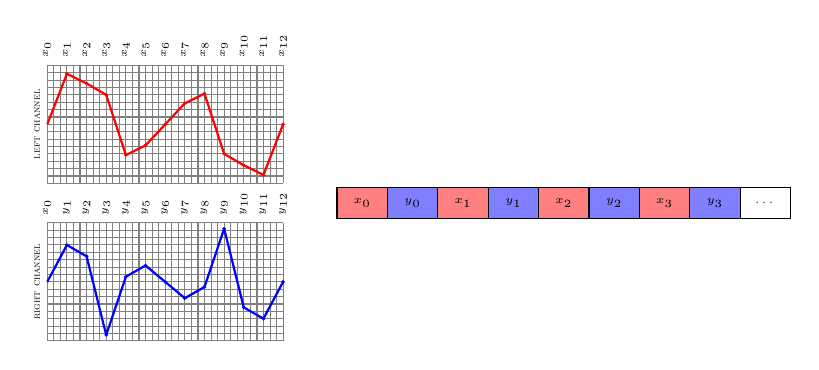
\begin{tikzpicture}[channel/.style={draw,font=\tiny,minimum height=5mm,minimum width=8mm},
                        channel 1/.style={channel,fill=red!50},
                        channel 2/.style={channel,fill=blue!50}]
      \begin{scope}[yshift=1cm,scale=.75,transform shape]
        \draw[thin,gray] (0,-1) grid[xstep=0.111cm,ystep=0.125cm] (4,1);
        \foreach[count=\i,
                 evaluate={0.7*sin(2*\x)+0.2*sin(5*\x)+0.3*sin(13*\x)} as \y,
                 remember=\y as \lasty (initially 0),
                 remember=\x as \lastx (initially 0)] \x in {30,60,...,360} {
          \draw[fill,red] (\x*0.0111,\y) circle [radius=0.02cm];
          \node[right,font=\tiny,rotate=90] at (\x*0.0111,1) {$x_{\i}$};
          \draw[thick,red] (\lastx*0.0111,\lasty) -- (\x*0.0111,\y);
        }
        \node[right,font=\tiny,rotate=90] at (0,1) {$x_0$};
        \node[rotate=90,anchor=south,font=\scshape\tiny] at (0,0) {left channel};
      \end{scope}
      \begin{scope}[yshift=-1cm,scale=.75,transform shape]
        \draw[thin,gray] (0,-1) grid[xstep=0.111cm,ystep=0.125cm] (4,1);
        \foreach[count=\i,
                 evaluate={0.6*sin(3*\x)+0.2*sin(2*\x)+0.3*sin(-17*\x)} as \y,
                 remember=\y as \lasty (initially 0),
                 remember=\x as \lastx (initially 0)] \x in {30,60,...,360} {
          \draw[fill,blue] (\x*0.0111,\y) circle [radius=0.02cm];
          \node[right,font=\tiny,rotate=90] at (\x*0.0111,1) {$y_{\i}$};
          \draw[thick,blue] (\lastx*0.0111,\lasty) -- (\x*0.0111,\y);
        }
        \node[right,font=\tiny,rotate=90] at (0,1) {$x_0$};
        \node[rotate=90,anchor=south,font=\scshape\tiny] at (0,0) {right channel};
      \end{scope}
      \begin{scope}[xshift=4cm,scale=.8,transform shape]
        \foreach \i in {0,...,3} {
          \node[channel 1] at (\i*0.8*2,0) {$x_{\i}$};
          \node[channel 2] at (\i*0.8*2+0.8,0) {$y_{\i}$};
        }
        \node[channel] at (8*0.8,0) {\dots};
      \end{scope}
    \end{tikzpicture}
  \end{center}
\end{frame}

\begin{frame}
  \frametitle{Dealing With Stereo Sound}
  \begin{center}
    \begin{tikzpicture}[milestone/.style={drop shadow,draw,fill=red!50,minimum height=7.5mm,minimum width=1cm,font=\tiny\scshape},
                        link/.style={-latex,thick},
                        arrow/.style={blue,ultra thick,-{Stealth[]}},
                        scale=.8,transform shape]
      \node[milestone] (uint8) at (0,0) {\texttt{Stream<uint8>}};
      \node[milestone] (int16) at ($ (uint8) + (2,1) $) {\texttt{Stream<int16>}};
      \node[milestone] (double) at ($ (uint8) + (4,0) $) {\texttt{Stream<double>}};
      \node[milestone] (double1) at ($ (double) + (3,1) $) {\texttt{Stream<double>}};
      \node[milestone] (double2) at ($ (double) + (3,-1) $) {\texttt{Stream<double>}};
      \node[milestone] (wave1) at ($ (double1) + (3,0) $) {\texttt{Wave}};
      \node[milestone] (wave2) at ($ (double2) + (3,0) $) {\texttt{Wave}};

      \coordinate (double top exit) at ($ (double.north) ! 0.5 ! (double.north east) $);
      \coordinate (double bottom exit) at ($ (double.south) ! 0.5 ! (double.south east) $);

      \draw[link] (uint8) |- (int16);
      \draw[link] (int16) -| (double);
      \draw[link] (uint8) -- (double);
      \draw[link] (double top exit) |- (double1);
      \draw[link] (double bottom exit) |- (double2);
      \draw[link] (double1) -- (wave1);
      \draw[link] (double2) -- (wave2);
    \end{tikzpicture}
  \end{center}
  \begin{itemize}
    \item In case of stereo sound, we need to split up the \texttt{Stream<double>} into two
    \item This way, we end up with one \texttt{Wave} per channel
  \end{itemize}
\end{frame}



%%% Local Variables:
%%% mode: latex
%%% TeX-master: "sound"
%%% End:

\subsection{The Way Back}

\frame{\tableofcontents[currentsubsection]}

\begin{frame}
  \frametitle{Writing WAV Files}
  \begin{center}
    \begin{tikzpicture}[milestone/.style={drop shadow,draw,fill=red!50,minimum height=7.5mm,minimum width=1cm,font=\tiny\scshape},
                        link/.style={-latex,thick},
                        arrow/.style={blue,ultra thick,-{Stealth[]}},
                        scale=.8,transform shape]
      \node[milestone] (wave1) {\texttt{Wave}};
      \node[milestone] (wave2) at ($ (wave1) + (0,-2) $) {\texttt{Wave}};
      \node[milestone] (double1) at ($ (wave1) + (3,0) $) {\texttt{Stream<double>}};
      \node[milestone] (double2) at ($ (wave2) + (3,0) $) {\texttt{Stream<double>}};
      \node[milestone] (double) at ($ (double1.east) ! 0.5 ! (double2.east) + (2,0) $) {\texttt{Stream<double>}};
      \node[milestone] (int16) at ($ (double) + (2,1) $) {\texttt{Stream<int16>}};
      \node[milestone] (uint8) at ($ (double) + (4,0) $) {\texttt{Stream<uint8>}};

      \coordinate (double top entry) at ($ (double.north) ! 0.5 ! (double.north west) $);
      \coordinate (double bottom entry) at ($ (double.south) ! 0.5 ! (double.south west) $);

      \draw[link] (wave1) -- (double1);
      \draw[link] (wave2) -- (double2);
      \draw[link] (double1) -| (double top entry);
      \draw[link] (double2) -| (double bottom entry);

      \draw[link] (double) -- (uint8);

      \draw[link] (double) |- (int16);
      \draw[link] (int16) -| (uint8);
    \end{tikzpicture}
  \end{center}
  \begin{itemize}
    \item We also need to be able to write WAV files
    \item The whole process needs to be reversed
  \end{itemize}
\end{frame}


%%% Local Variables:
%%% mode: latex
%%% TeX-master: "sound"
%%% End:






%%% Local Variables:
%%% mode: latex
%%% TeX-master: "sound"
%%% End:
